\appendix
\chapter{Pseudocode}
\section{Region Growing}
\begin{figure}[H]
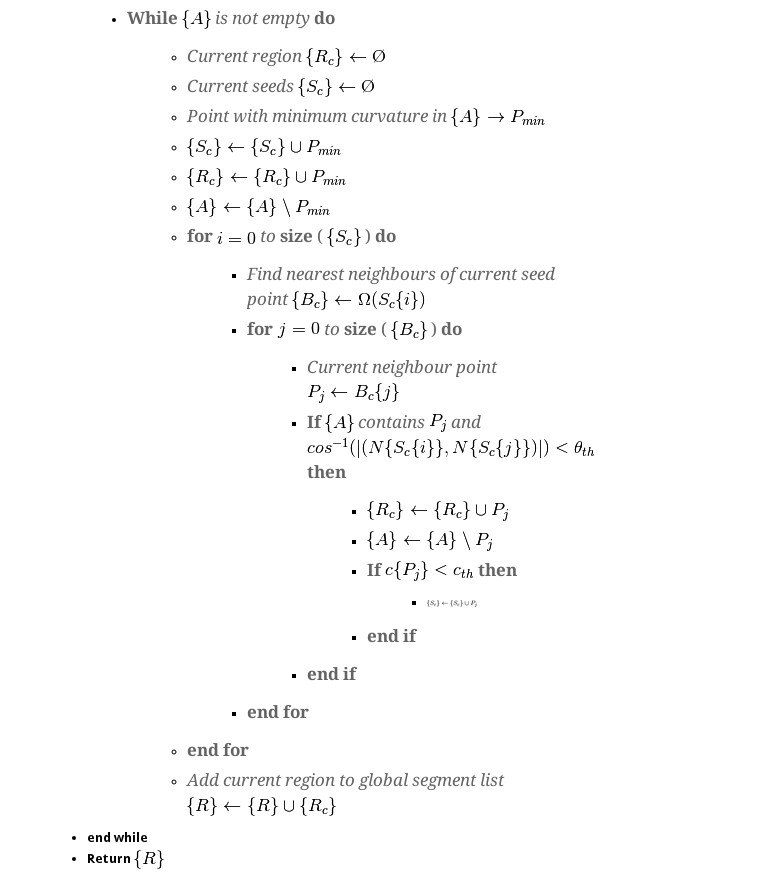
\includegraphics[width=.9\linewidth]{Includes/images/RegionGrowingPseudocode}
\end{figure}

\section{RANSAC}

\begin{lstlisting}
Given:
data - a set of observed data points
model - a model that can be fitted to data points
n - the minimum number of data values required to fit the model
k - the maximum number of iterations allowed in the algorithm
t - a threshold value for determining when a data point fits a model
d - the number of close data values required to assert that a model fits well to data
Return:
bestfit - model parameters which best fit the data (or nil if no good model is found)
iterations = 0
bestfit = nil
besterr = something really large
while iterations < k {
	maybeinliers = n randomly selected values from data
	maybemodel = model parameters fitted to maybeinliers
	alsoinliers = empty set
	for every point in data not in maybeinliers {
		if point fits maybemodel with an error smaller than t
		add point to alsoinliers
	}
	if the number of elements in alsoinliers is > d {
		% this implies that we may have found a good model
		% now test how good it is
		bettermodel = model parameters fitted to all points in maybeinliers and alsoinliers
		thiserr = a measure of how well model fits these points
		if thiserr < besterr {
			bestfit = bettermodel
			besterr = thiserr
		}
	}
	increment iterations
}
return bestfit


\end{lstlisting}


\chapter{GTL Full Results}

ADD TEXT ABOUT THESE IMAGES

\begin{figure}[H]
\centering
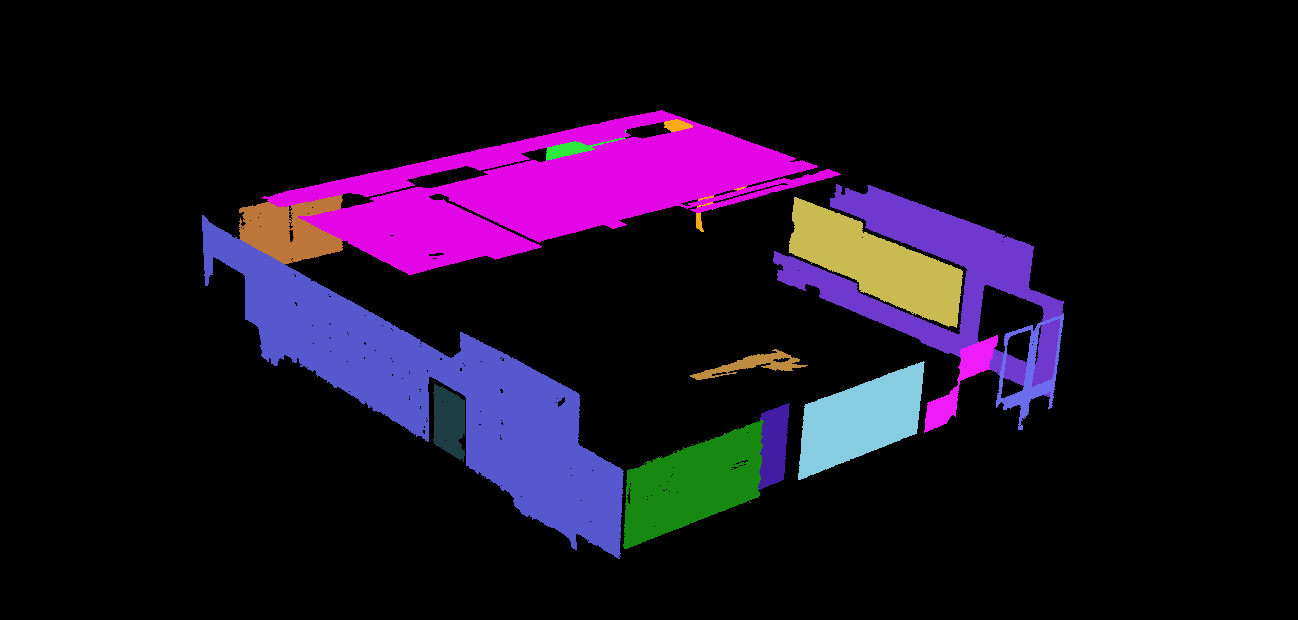
\includegraphics[width=1\linewidth]{Includes/images/Appendix/GTL-Full-seg}
\caption{}
\label{fig:GTL-Full-seg}
\end{figure}

\begin{figure}[H]
	\centering
	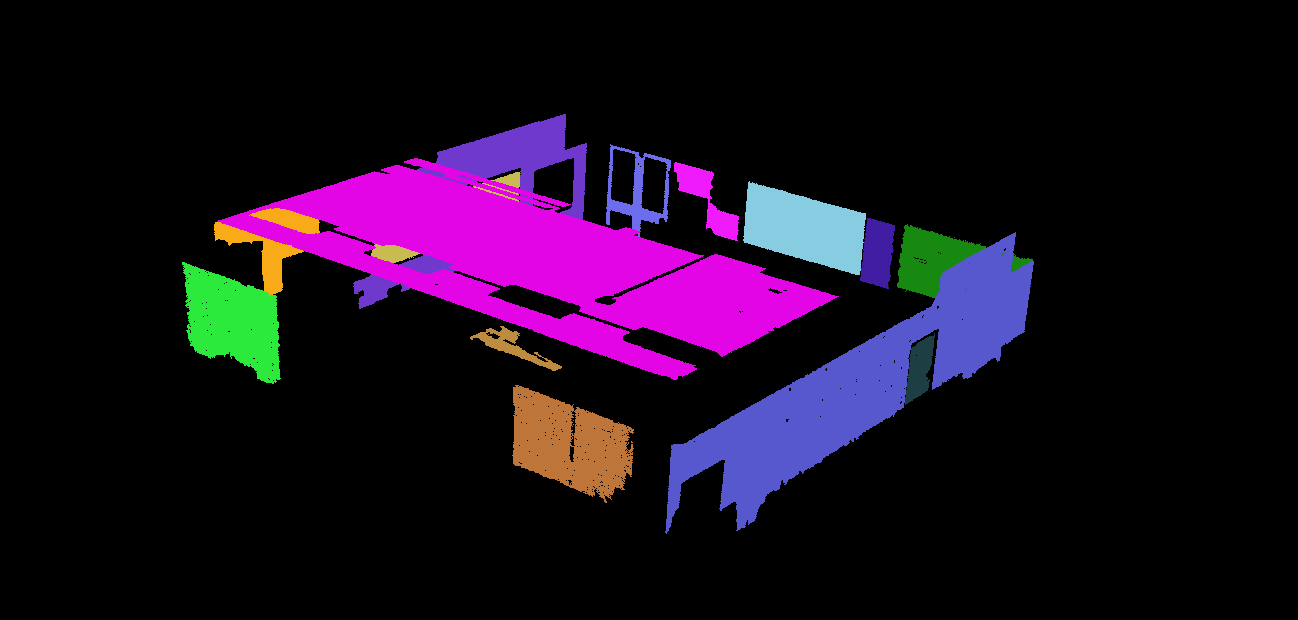
\includegraphics[width=1\linewidth]{Includes/images/Appendix/GTL-Full-seg2}
	\caption{}
	\label{fig:GTL-Full-seg2}
\end{figure}


